% ****** Start of file apssamp.tex ******
%
%   This file is part of the APS files in the REVTeX 4.1 distribution.
%   Version 4.1r of REVTeX, August 2010
%
%   Copyright (c) 2009, 2010 The American Physical Society.
%
%   See the REVTeX 4 README file for restrictions and more information.
%
% TeX'ing this file requires that you have AMS-LaTeX 2.0 installed
% as well as the rest of the prerequisites for REVTeX 4.1
%
% See the REVTeX 4 README file
% It also requires running BibTeX. The commands are as follows:
%
%  1)  latex apssamp.tex
%  2)  bibtex apssamp
%  3)  latex apssamp.tex
%  4)  latex apssamp.tex
%
\documentclass[%
 reprint,
%superscriptaddress,
%groupedaddress,
%unsortedaddress,
%runinaddress,
%frontmatterverbose, 
%preprint,
showpacs,
%,preprintnumbers,
%nofootinbib,
%nobibnotes,
%bibnotes,
 amsmath,amssymb,
 aps,
%pra,
%prb,
%rmp,
%prstab,
%prstper,
%floatfix,
]{revtex4-1}

\usepackage{graphicx}% Include figure files
\usepackage{dcolumn}% Align table columns on decimal point
\usepackage{bm}% bold math
\usepackage{subfig}

%\usepackage{hyperref}% add hypertext capabilities
%\usepackage[mathlines]{lineno}% Enable numbering of text and display math
%\linenumbers\relax % Commence numbering lines
%
%\usepackage[showframe,%Uncomment any one of the following lines to test 
%%scale=0.7, marginratio={1:1, 2:3}, ignoreall,% default settings
%%text={7in,10in},centering,
%%margin=1.5in,
%%total={6.5in,8.75in}, top=1.2in, left=0.9in, includefoot,
%%height=10in,a5paper,hmargin={3cm,0.8in},
%]{geometry}

\begin{document}
%%% new commands and macros %%%%%%%%%%%%%%%%%%%%%%%%%%%%%%%%%%%%%%%%%%%
\newlength{\figwidth}
\setlength{\figwidth}{0.9\columnwidth}

\newlength{\qfigheight}
\setlength{\qfigheight}{0.25\textheight}

\newlength{\hfigheight}
\setlength{\hfigheight}{0.5\textheight}

\newcommand{\dedicationfont}{\fontencoding{T1}\fontfamily{anttlc}\fontseries{m}\fontshape{n}\fontsize{12}{15}\selectfont}

\newcommand{\acro}[1]{#1\@}
\newcommand{\abbr}[1]{\textsc{\texttt{#1}}}
\newcommand{\abbrlc}[2]{\textsc{\texttt{#1}}\texttt{#2}}
\newcommand{\desg}[1]{\texttt{#1}}
\newcommand{\todo}[1]{\textbf{\uppercase{\emph{#1}}}} %\textcolor{Orange}{#1}}}


%Some variables
%
%
\def\g12{\emph{g12}}

\def\G11{\emph{g11}}
\def\clas{\abbr{CLAS }}

\def\Lqcd{\mathcal{L}_{\mathtt{QCD}}}
\def\qfield{\psi}
\def\qbarfield{\overline{\psi}}

\def\grpath{/Users/michaelkunkel/WORK/GIT_HUB/THESIS/figures/print}
\def\figures{/Users/michaelkunkel/WORK/GIT_HUB/THESIS/figures/print}
\def\tablepath{../../}
\newcommand{\bank}[4]{$\mathtt{#1}^{#2}_{#3}\lbrack\mathtt{#4}\rbrack$}

\def\ith{$i$\textsuperscript{th}}

\def\um{{\text{$\mu$}}m}

%\def\coloronline{(Color online.)\ }
\def\coloronline{}

%%% particles
\def\p{\mathrm{p}}
\def\n{\mathrm{n}}
\def\Kp{\mathrm{K}^{+}}
\def\Km{\mathrm{K}^{-}}
\def\K0{\mathrm{K}^{0}}
\def\Y{\mathrm{Y}}
\def\epos{\mathrm{e}^{+}}
\def\eneg{\mathrm{e}^{-}}
\def\gamstar{\mathrm{$\gamma$}^{*}}
\def\piup{$\pi$}
\def\gammaup{$\gamma$}
%%% TAGGER and RF related times
\def\trf{t_{\mathtt{RF}}}
\def\ttag{t_{\mathtt{TAG}}}
\def\ttagrf{t_{\mathtt{TAG,RF}}}
\def\tprop{t_\mathrm{prop}}
\def\ttrigoffset{t_{\mathrm{trigger-offset}}}

%%% BEAM energy
\def\ebeam{E_{\mathrm{beam}}}

%%% Beta
\def\betasttof{\beta_{\mathtt{ST-TOF}}}
\def\betatof{\beta_{\mathrm{vtx}\mathtt{-TOF}}}
\def\betap{\beta_{p}}

%%% path lengths
\def\lst{\ell_{\mathtt{ST}}}
\def\ltof{\ell_{\mathtt{TOF}}}
\def\lsttof{\ell_{\mathtt{ST-TOF}}}

%%% raw subsystem times
\def\tst{t_{\mathtt{ST}}}
\def\ttof{t_{\mathtt{TOF}}}
\def\dtsttof{\Delta t_{\mathrm{ST-TOF}}}

%%% vertex times
\def\tv{t_{\mathrm{vtx}}}
\def\tvtagrf{t_{\mathrm{vtx}}(\mathtt{TAG_{RF}})}
\def\tvst{t_{\mathrm{vtx}}(\mathtt{ST})}

\def\adcst{\mathtt{ADC}_{\mathtt{ST}}}

\newcommand{\bra}[1]{\left<#1\right|}
\newcommand{\ket}[1]{\left|#1\right>}
\newcommand{\braket}[2]{\left<#1\middle|#2\right>}
\def\piz{$\mathrm{\pi^{0}}\ $}
\def\epem{$e^+e^-\ $}
\preprint{APS/123-QED}

\title{Photoproduction of the $\pi^0$ meson from 3.9 - 5.5~GeV with a comparison to the Regge Model}% Force line breaks with \\
%\thanks{A footnote to the article title}%

\author{Michael C. Kunkel}
 \altaffiliation[Now at ]{Forschungszentrum J\"ulich.}%Lines break automatically or can be forced with \\
%\author{Second Author}%
% \email{Second.Author@institution.edu}
\affiliation{%Physics Department, Old Dominion University.
 Physics Department, Old Dominion University. \\
% This line break forced with \textbackslash\textbackslash
}%

\collaboration{CLAS Collaboration}%\noaffiliation

%\author{Charlie Author}
% \homepage{http://www.Second.institution.edu/~Charlie.Author}
%\affiliation{
% Second institution and/or address\\
% This line break forced% with \\
%}%
%\affiliation{
% Third institution, the second for Charlie Author
%}%
%\author{Delta Author}
%\affiliation{%
% Authors' institution and/or address\\
% This line break forced with \textbackslash\textbackslash
%}%
%
%\collaboration{CLEO Collaboration}%\noaffiliation

\date{\today}% It is always \today, today,
             %  but any date may be explicitly specified

\begin{abstract}
Exclusive neutral pion photoproduction ($\gamma p \rightarrow p \pi^0$) was measured in the CLAS detector at the Thomas Jefferson National Facility. The experiment employed a 1.1-5.5~GeV bremsstrahlung photon beam from 5.6~GeV electron beam created in the Continuous Electron Beam Accelerator Facility (CEBAF). The photon beam energy was impinged on a liquid hydrogen target. The neutral pions were detected via external conversion, $\pi^0 \rightarrow \gamma \gamma \rightarrow e^+e^-\gamma$, and subsequent Dalitz decay, $\pi^0 \rightarrow \gamma^* \gamma \rightarrow e^+e^-\gamma$. Measured differential cross-sections, $\frac{d\sigma}{dt}$ and $\frac{d\sigma}{d\cos \theta}$ are compared with Regge theory. The Regge theoretical calculations underestimate the differential cross sections between 3.9 and 4.6~GeV, but agree with data at photon energies 4.6-5.4~GeV.   

%\begin{description}
%\item[Usage]
%Secondary publications and information retrieval purposes.
%\item
%\pacs{13.20.Cz, 13.25.Cq, 13.30.Ce,  13.60.Le, 14.40.0n}
%%\pacs{PACS numbers: 13.20.Cz, 13.25.Cq, 13.30.Ce,  13.60.Le, 14.40.0n}% PACS, the Physics and Astronomy
%May be entered using the \verb+\pacs{#1}+ command.
%\item[Structure]
%You may use the \texttt{description} environment to structure your abstract;
%use the optional argument of the \verb+\item+ command to give the category of each item. 
%\end{description}
\end{abstract}

\pacs{13.20.Cz, 13.25.Cq, 13.30.Ce,  13.60.Le, 14.40.0n}% PACS, the Physics and Astronomy
                             % Classification Scheme.
%\keywords{Suggested keywords}%Use showkeys class option if keyword
                              %display desired
\maketitle

%\tableofcontents
\section{\label{sec:level1}Introduction}
In hadron physics, photoproduction of single pion is essential to understand the photon-nucleon vertex. At low energies, the photon-nucleon coupling establishes excited nucleon resonances which has been at the forefront of physics ''missing resonances'' search. At high energies single pion photoproduction can be used to test predictions of Regge theory, in which recent calculations~\cite{JPAC} have shown to describe the presented data well. Furthermore, these measurements have shown that the differential cross section for single pion photoproduction at fixed c.m. angles, $\theta_{c.m.}$, of $70^{\circ}$, $90^{\circ}$ and $110^{\circ}$ seem to scale as $\frac{d\sigma}{dt} \sim s^{2-n}f(\theta_{c.m.})$, where $s$ and $t$ are the Mandelstam variables and $n$ is the total number of interacting elementary fields in the initial and final state of the reaction. This is predicted by the constituent counting rule~\cite{scaling1,scaling2} and exclusive measurements in $pp$ and  $\bar{p}p$ elastic scattering~\cite{scalingexp5, scalingexp7}, meson-baryon $M p$ reactions~\cite{scalingexp7}, and photoproduction $\gamma N$~\cite{scalingexp2, scalingexp3, scalingexp4, scalingexp6, scalingexp8, scalingexp9, scalingexp10, scalingexp11} agree well with this rule. The following paper details the CLAS g12 experiment, the extraction of single neutral pion photoproduction from data, the differential cross-sections through the entire beam energy range of the g12 experiment, a comparison of the differential cross-section with existing world data, and a comparison to the constituent counting rule. 



\section{Experimental Setup}\label{sec:setup}
	The measurements used for this analysis was taken with the \abbr{CLAS} detector at Hall B at the Thomas Jefferson National Accelerator Facility \abbr{TJNAF} located in 
	Newport News, Virginia. The \g12 experiment is a photoproduction experiment, it ran during March - June 2008 with a total of 44 days of good beam time. It collected over 
	128~TB of raw data that consisted of $26\cdot 10^9$ events, with an integrated luminosity of 68~pb$^{-1}$. The photon beam was produced by impinging a $5.715$~GeV 
	electron beam, at 65nA, on a Au radiator of $10^{-4}$ radiation length. Photons in the energy range from 20\% to 95\% of the electron beam
	energy were tagged, resulting in a photon beam energy range of 1.1-5.5~GeV. This photon beam was then collimated before being introduced onto a $\ell H_2$ target 40~cm in 
	length along the z-direction and 2~cm radius. The placement of the target was 90~cm upstream from \abbr{CLAS} center (toward Au radiator), this increased the acceptance 
	of particles in the forward direction. During the runtime of \g12, the Cherenkov detectors were filled with perfluorobutane ($\mathrm{C_4F_{10}}$) allowing for electron/positron 
	detection. The experiment had a dedicated trigger, amongst 9 other triggers, that consisted of Cherenkov Counter(\abbr{CC}) and Electro-magnetic Calorimeter(\abbr{EC}) 
	coincidence hits for the entire beam energy range. With proper cuts on the \abbr{CC} and \abbr{EC} a $\pi/e$ rejection of $10^6$ for $e^{\pm}$ pairs was established.
\section{Event Selection}\label{sec:evnt}
	Pions were skimmed initially and then re-identified as leptons by changing the mass of the pion. This method is sufficient when the decaying particle's mass, i.e. $m_{\pi^0}$, 
	is less than that of $\pi^{\pm}$. If the event satisfied the requirements listed in Table~\ref{tab:skim.requirements}, then all timing, momentum and vertex information was 
	outputted as well as \abbr{CC} and \abbr{EC} information to be used to identify leptons, as discussed in Sec~\ref{sec:analysis.pid}. To reduce the size of the data set, a cut 
	was placed on the total missing mass of $\gamma p \to p \pi^{+} \pi^{-}$ to be less than 275~MeV. This cut was broad enough to not interfere with \piz selection from single 
	\piz production i.e. $\gamma p \to p \pi^{0}$ when assigned the pion the lighter mass of a electron/positron. This broad cut also does not interfere with \piz production from 
	light meson decay, i.e $\gamma p \to p \omega \to p \pi^{+} \pi^{-} \pi^{0}$. 
	\begin{table}[h!]
\begin{minipage}{\textwidth}
\begin{center}
\begin{singlespacing}
\caption[Skim requirements]{\label{tab:skim.requirements}Requirements of initial skim \vspace{0.75mm}} %\vspace{0.75mm}

\begin{tabular}{lr}

\hline
Requirement & \quad \quad Section Discussed \\
\hline
One in-time beam photon &  Sec.~\ref{sec:analysis.beam} \\ 
One proton & Sec.~\ref{sec:data.cook} \\
One $\pi^+$ or \emph{``unknown''} of q$^+$ & Sec.~\ref{sec:data.cook} \\
One $\pi^-$ or \emph{``unknown''} of q$^-$ & Sec.~\ref{sec:data.cook} \\
\hline \hline
\end{tabular}

\end{singlespacing}
\end{center}
\end{minipage}
\end{table}
\vspace{20pt}
\section{\label{sec:level1}Particle Identification}
Write 
%\section{\label{sec:analysis.simulation}Monte-Carlo}
	There are certain kinematic regions of \abbr{CLAS} in which physics events are not being recorded properly i.e.~the area dividing each sector in \abbr{CLAS}. Furthermore each sector in \abbr{CLAS} is asymmetric in the acceptance of events due to subsystem inefficiencies such as inoperable \abbr{DC} wires, \abbr{PMT} inefficiencies, dead scintillator strips the the \abbr{TOF} and \abbr{ST} subsystems. When a triggered event is recorded and reconstructed these asymmetric inefficiencies factors are reflected and must be carefully understood because these factors are properties of the \abbr{CLAS} detector and independent of any physics that occurred. To properly understand the detector effects on the data, \abbr{CLAS} utilizes a \abbr{GEANT} simulation package know as \abbr{GSIM}. To prepare an event for \abbr{GSIM} the program \abbr{GAMP2PART} converts a text file, containing the 4-momentum of the generated event, into a suitable file format for \abbr{GSIM}. \abbr{GSIM} then simulates the passage of these particles through the \abbr{CLAS} detector and generates the associated \abbr{ADC} and \abbr{TDC} information from detector hits. \abbr{GSIM} takes into account detector inefficiencies described in the \abbr{\texttt{CLAS\_CALDB\_RUNINDEX}}. The \abbr{CLAS\_CALDB\_RUNINDEX} is an array of information about each subsystem's inefficiency that was derived during the \g12 calibration process. The \abbr{GSIM} simulated hits are then ``post-processed'' by smearing the \abbr{TDC} and \abbr{ADC} hits to imitate the observed resolution of the detector subsystems using the program \abbr{GPP} (\abbr{GSIM} post-processor). \abbr{GPP} also removes detector hits due to inefficient \abbr{DC} wires.
	
	 The acceptance for the cross-sections presented in this work was measured using phase-space Monte-Carlo (\abbr{MC}\label{abbr:mc}) simulation, using PLUTO++~\cite{PLUTO} as the generator, for the reaction channels,
	\begin{subequations}
		\begin{align}
				\gamma \p \rightarrow & \ p \pi^{0} \nonumber \\[-0.4em]
				& \ \hookrightarrow p \gamma \gamma \nonumber \\[-0.4em]
				& \qquad \hookrightarrow p e^+ e^- \gamma
				\label{eq:simproduct1}
			\end{align}
			\begin{align}
				\gamma \p \rightarrow & \ p \pi^{0} \nonumber \\[-0.4em]
				& \ \hookrightarrow p e^+ e^- \gamma.
				\label{eq:simproduct2}
			\end{align}
		\end{subequations} 
		A total of events, $N_g$, was generated and this number was weighted by the relative branching ratios found in Table~\ref{tab:targetspecs} to resemble the conditions of the data. The number of events generated for the reaction channel~\ref{eq:simproduct1} can be found in Table~\ref{tab:simnumspecs} as $N_c$. The number of events generated for the reaction channel n~\ref{eq:simproduct2} can be found in Table~\ref{tab:simnumspecs} as $N_d$.
		\begin{table}[h!]
\begin{minipage}{\textwidth}
\begin{center}
\begin{singlespacing}

\caption[Generated Quantities]{\label{tab:simnumspecs}Number of generated events in each decay spectrum}

\begin{tabular}{c|c|c}

%\hline \hline
%
%operation & \multicolumn{3}{c}{Generation} \\
%charge & I & II & III \\
\hline
Quantity & Value & Description\\
\hline

$N_g$ & $2.39869 \cdot 10^9$ & Total number of \piz events generated \\
$N_c$ & $2.37039 \cdot 10^9$ &  Total number of \piz $\rightarrow \gamma \gamma$ events generated\\
$N_d$ & $2.80647 \cdot 10^7$ & Total number of \piz $\rightarrow e^+ e^- \gamma$ generated\\
\hline \hline
\end{tabular}

\end{singlespacing}
\end{center}
\end{minipage}
\end{table}
\vspace{20pt}
		After the events are generated, they are inputted into the \abbr{CLAS} simulation chain \abbr{GAMP2BOS}\label{abbr:gamp2bos}, \abbr{GSIM}\label{abbr:gsim}, \abbr{GPP}\label{abbr:gpp}, and then reconstructed with the same program used to reconstruct the data, \abbrlc{}{a1c}\label{abbr:a1c}, all programs in the simulation chain use the parameters and the run index described above. Once the events are processed through \abbrlc{}{a1c}, the cuts described in Secs.~\ref{sec:analysis.data.reduction}, ~\ref{sec:analysis.fitting.compare}, are applied as they are to the real data. The acceptance $\eta(E_\gamma,\theta^{\pi^0}_{C.M.})$ is then determined by adding the simulations for the conversion and the dalitz, then for photon energy bins of 25 MeV increments and $\Delta\cos\theta^{\pi^0}_{C.M.} = 0.0125$ increments, the ratio of reconstructed events ($N_R$) to generated events ($N_G$) yields,
		\begin{equation}\label{eq:acceptance}
		\eta(E_\gamma,\cos\theta^{\pi^0}_{C.M.}) = \frac{N_R(E_\gamma,\cos\theta^{\pi^0}_{C.M.})}{N_G(E_\gamma,\cos\theta^{\pi^0}_{C.M.})} \ .
		\end{equation}
		The $\Delta\cos\theta^{\pi^0}_{C.M.}$ binning in the acceptance is a factor of 2.4 finer than the smallest $\Delta\cos\theta^{\pi^0}_{C.M.}$ increment used in the cross-section measurement. If an accurate physics model for the generator had been used, as was in Sec.~\ref{sec:analysis.simulation}, the binning for the acceptance  would not have had to be so fine.
	
	
%	\subsection{Simulating the Lepton Trigger}\label{sec:analysis.accept.trigger}
%		During the collection process, for an event to be written by the \abbr{DAQ} it must have passed at least one of the trigger ``bits" defined in Sec.~\ref{sec:clas.g12.conditions.data}. As discussed in Sec.~\ref{sec.data.trig.lepton}, the process of lepton triggering required a coincidence between the \abbr{EC} and the \abbr{CC} subsystems. This coincidence was established by using the voltage sum of the \abbr{CC} for a sector and the voltage sum of the \abbr{EC} for the same sector and comparing each sum to a preset threshold described in Table~\ref{tab:data.ecccthresh}. However when \abbr{GSIM} simulates tracks through the \abbr{CC} and \abbr{EC}, it does not account for the minimum voltage threshold that was required for data collection, moreover the simulation of the trigger must match the trigger efficiency discussed in Sec.~\ref{sec:analysis.trigger.verify}.
%		
%		Simulation of the \abbr{CC} and \abbr{EC} trigger ``bit 6'', Sec.~\ref{sec.data.trig.lepton}, was performed by writing an algorithm that attempted to mimic the method in which triggered data was recorded. To accomplish this a modified function, written by Simeon McAleer from FSU, was written into the simulation reconstruction algorithm. The routine returned the sector and a boolean of 0 or 1 (pass or fail), that simulated the trigger based on the following criteria;
%		\begin{enumerate}\label{trig:sim.all}
%			\item The sector with the highest EC summed energy over threshold. \label{trig:sim.ECtot} 
%			\item The sector with the highest EC Inner Layer summed energy over threshold. \label{trig:sim.ECinner} 
%			\item The sector with the highest CC summed energy over threshold. \label{trig:sim.CCtot} 
%			\item All three above conditions must be in same sector.
%		\end{enumerate}
%		Thresholds as described in Table~\ref{tab:data.ecccthresh} are 80~mV, 60~mV and 20~mV for \abbr{EC} \emph{inner}, \abbr{EC}\emph{total} and CC respectively. The \abbr{CC} trigger threshold was applied to groups of eight \abbr{CC} \abbr{PMT}s, called ``sim bits''. The ``sim bits'' were staggered by four \abbr{PMT}s so that each \abbr{PMT} goes into two ``sim bits'', after which all ``sim bits'' were ``\emph{OR}'''d together. If any ``sim bit'' calculated as above threshold, that specific sector was then compared to the remaining sectors to establish the condition listed in~\ref{trig:sim.CCtot}.
%		
%		The \abbr{EC} \emph{inner} and \abbr{EC} \emph{total} trigger thresholds were applied to all \abbr{EC} strips in a sector. This was done by summing over the energy for every strip in every orientation of the \abbr{EC} per sector. If the energy summation for the \abbr{EC} \emph{inner} was above threshold,   that specific sector was then compared to the remaining sectors to establish the condition listed in~\ref{trig:sim.ECinner}. If the energy summation for the \abbr{EC} \emph{total} was above threshold, that specific sector was then compared to the remaining sectors to establish the condition of the sector with the highest EC summed energy over threshold.
%		
%		\subsubsection{Validity of Trigger Simulation}
%			The actual triggered data could have been triggered by the following sceneries;
%			\begin{enumerate}\label{trig:get.all}
%				\item $e^-$ \abbr{CC} and \abbr{EC} hit above preset thresholds,
%				\item $e^+$ \abbr{CC} and \abbr{EC} hit above preset thresholds,
%				\item $e^-$ \abbr{CC} hit above preset thresholds and $e^+$ \abbr{EC} hit above preset thresholds in the same sector, 
%				\item $e^-$ \abbr{EC} hit above preset thresholds and $e^+$ \abbr{CC} hit above preset thresholds in the same sector. 
%			\end{enumerate}
%			The lepton trigger ``bit 6" was 100\% efficient (see Sec.~\ref{sec:analysis.trigger.verify}) when the data was cut using all the conditions listed above (1, 2, 3, 4) using an ``OR" flag. This means that a $\gamma p \to p e^+ e^-$ event must satisfy at least one of the listed conditions. The reduction in events when at least one of the conditions was satisfied was 69.91\%. Prior to simulating the trigger, cutting the \abbr{MC} with the listed conditions reduced the event yield by 81.91\%. Simulating the trigger and cutting on the \abbr{MC} events with the listed conditions reduced that event yield to 69.48\%. This indicates that the trigger simulation is properly mimicking the trigger configuration used when data is collected. 
%
%\section{PLUTO++ Event Generator}\label{sec:pluto}
%
%	Pluto~\cite{PLUTO} is a Monte-Carlo event generator designed for the study of hadronic interactions and heavy ion reactions in \abbr{HADES}, \abbr{FAIR} and upcoming \abbr{PANDA} collaborations. The versatility of Pluto enables its use as an event generator for photoproduction in \abbr{CLAS}. For hadronic interactions, Pluto can generate interactions from pion production threshold to intermediate energies of a few~GeV per nucleon. The entire software package is based on ROOT and uses ROOT's embedded C++ interpreter to control the generation of events. Programming event reaction can be set up with a few lines of ROOT macro code without detailed knowledge of programming. Some features in Pluto are, but not limited to;
%	\begin{itemize}
%		\item Ability to generate events in phase space.
%		\item Ability to generate events with a continuous bremsstrahlung photon beam.
%		\item Ability to generate events weighted by a user defined $t$-slope.
%		\item Ability to generate events weighted by a user defined cross-section.
%		\begin{itemize}
%			\item Total cross section can be inputted via functional form or histogram.
%			\item Differential cross sections can be inputted via functional forms or histograms for specific beam energies up to 110 histograms relating to intervals of beam energy.
%		\end{itemize}
%		\item Ability to generate events that decay via already established physics parameters, i.e.~transition form factors.
%		\item Ability to generate events that decay via modified established physics parameters.
%		\item Ability to generate events with multiple production channels, weighted by user inputted cross-section probability.
%		\item Ability to generate events with multiple decay channels, weighted by user inputted branching ratio.
%		\item Ability to perform vertex smearing.
%		\item Ability to create virtual detectors.
%	\end{itemize}
%	
	For the analysis presented in this work, Pluto was used in conjunction with known differential cross sections to verify simulation momentum smearing and tagger resolution, Sec.~\ref{sec:analysis.simsmear.verify}. Pluto was also utilized as a phase space generator in this analysis, to perform a ``tune'' on the kinematic fitter, Sec.~\ref{sec:analysis.fitting}, to calculate the acceptance corrections Sec.~\ref{sec:results.acceptance}, and to calculate the normalization Sec.~\ref{sec:results.normalization}.
%\section{\label{sec:level1}Systematic Uncertainties}
 Systematic errors are caused the controls of the experiment, such as flux, simulation, density and length of the $\ell H_2$ target and also systematic errors are caused by various analytical tools used, such as the kinematic fitter.
 \subsection{Branching Ratio Systematic Uncertainty}
 The branching ratios for the two topologies used to measure the cross-section were obtained from \abbr{PDG}\label{abbr:pdg}~\cite{pdg} and are listed again in Table~\ref{tab:brspecs} with their associated errors. Uncorrelated quantities that are summed as,
 \begin{align}
 	f = \sum_{i = 1}^{M}a_iP_i  
 \end{align}
 have errors as
 \begin{align}
 	\sigma_f = \sqrt{\sum_{i = 1}^{M}\left(a_i\sigma_i\right)^2}.  
 \end{align}
 Therefore
 \begin{align}
 	\frac{\Gamma}{\Gamma_{tot}} &  = \frac{\Gamma_{\pi^{0}\rightarrow e^{+}e^{-}\gamma}}{\Gamma_{tot}} + \frac{\Gamma_{\pi^{0}\rightarrow \gamma \gamma \to e^{+}e^{-}\gamma}}{\Gamma_{tot}}  \\ & = \frac{\Gamma_{\pi^{0}\rightarrow e^{+}e^{-}\gamma}}{\Gamma_{tot}} + \frac{\Gamma_{\pi^{0}\rightarrow \gamma \gamma}P(\gamma \to  e^{+}e^{-})}{\Gamma_{tot}} \ ,
 \end{align}
 where $P(\gamma \to  e^{+}e^{-})$ is the probability of photon conversion into $e^+e^-$. To measure $P(\gamma \to  e^{+}e^{-})$, the acceptance for conversion ($P(\gamma \to  e^{+}e^{-})\cdot\eta_{e^+e^-}$) is divided by the acceptance for Dalitz ($\eta_{e^+e^-}$). Fig.~\ref{fig:convprob_all} shows that the conversion probability depends on incident photon energy. A maximum probability of 8\%  per-photon was measured, shown in Fig~\ref{fig:convprob_II} top left plot. 
 \begin{figure}[h!]\begin{center}
 		\subfloat[Probability of Photon Conversion vs. $\cos\theta$][]{ %Feynman diagram of \piz two photon decay
 			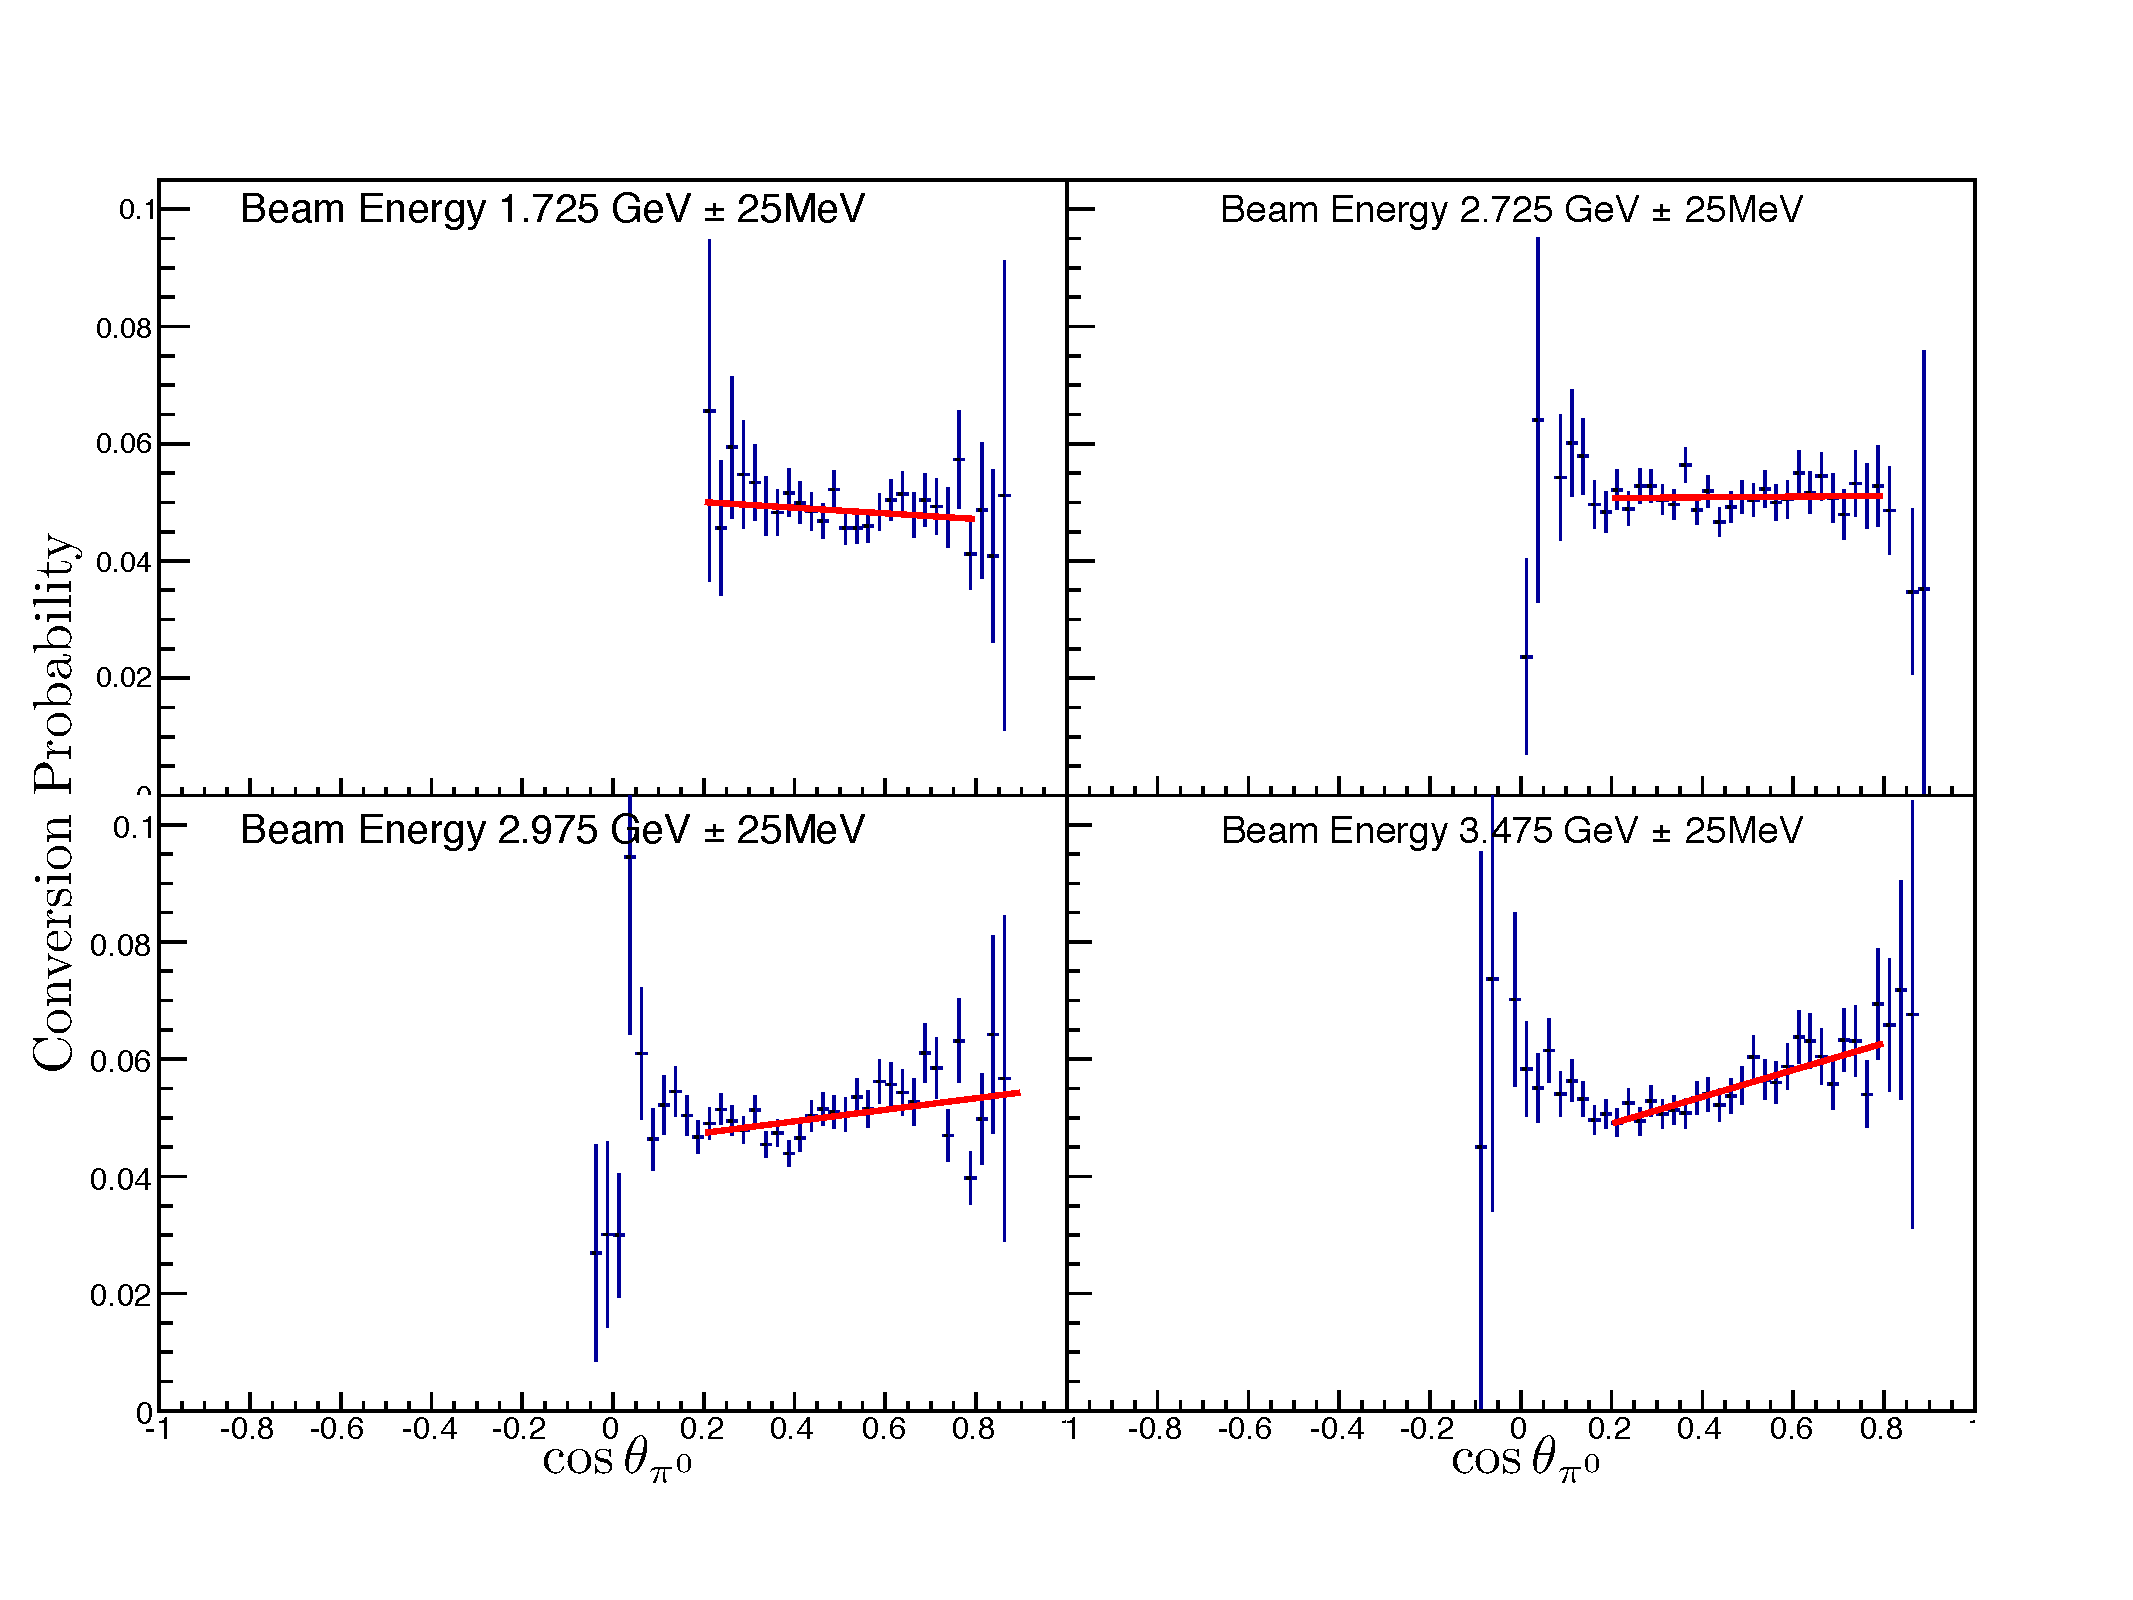
\includegraphics[width=\figwidth,height=\qfigheight]{\grpath/analysis/BRANCHING_RATIO/Converion_Probability_fix.pdf}\label{fig:convprob_I}
 		}\\
 		\subfloat[Probability of Photon Conversion vs. $\cos\theta$][]{ %Feynman diagram of \piz Dalitz decay
 			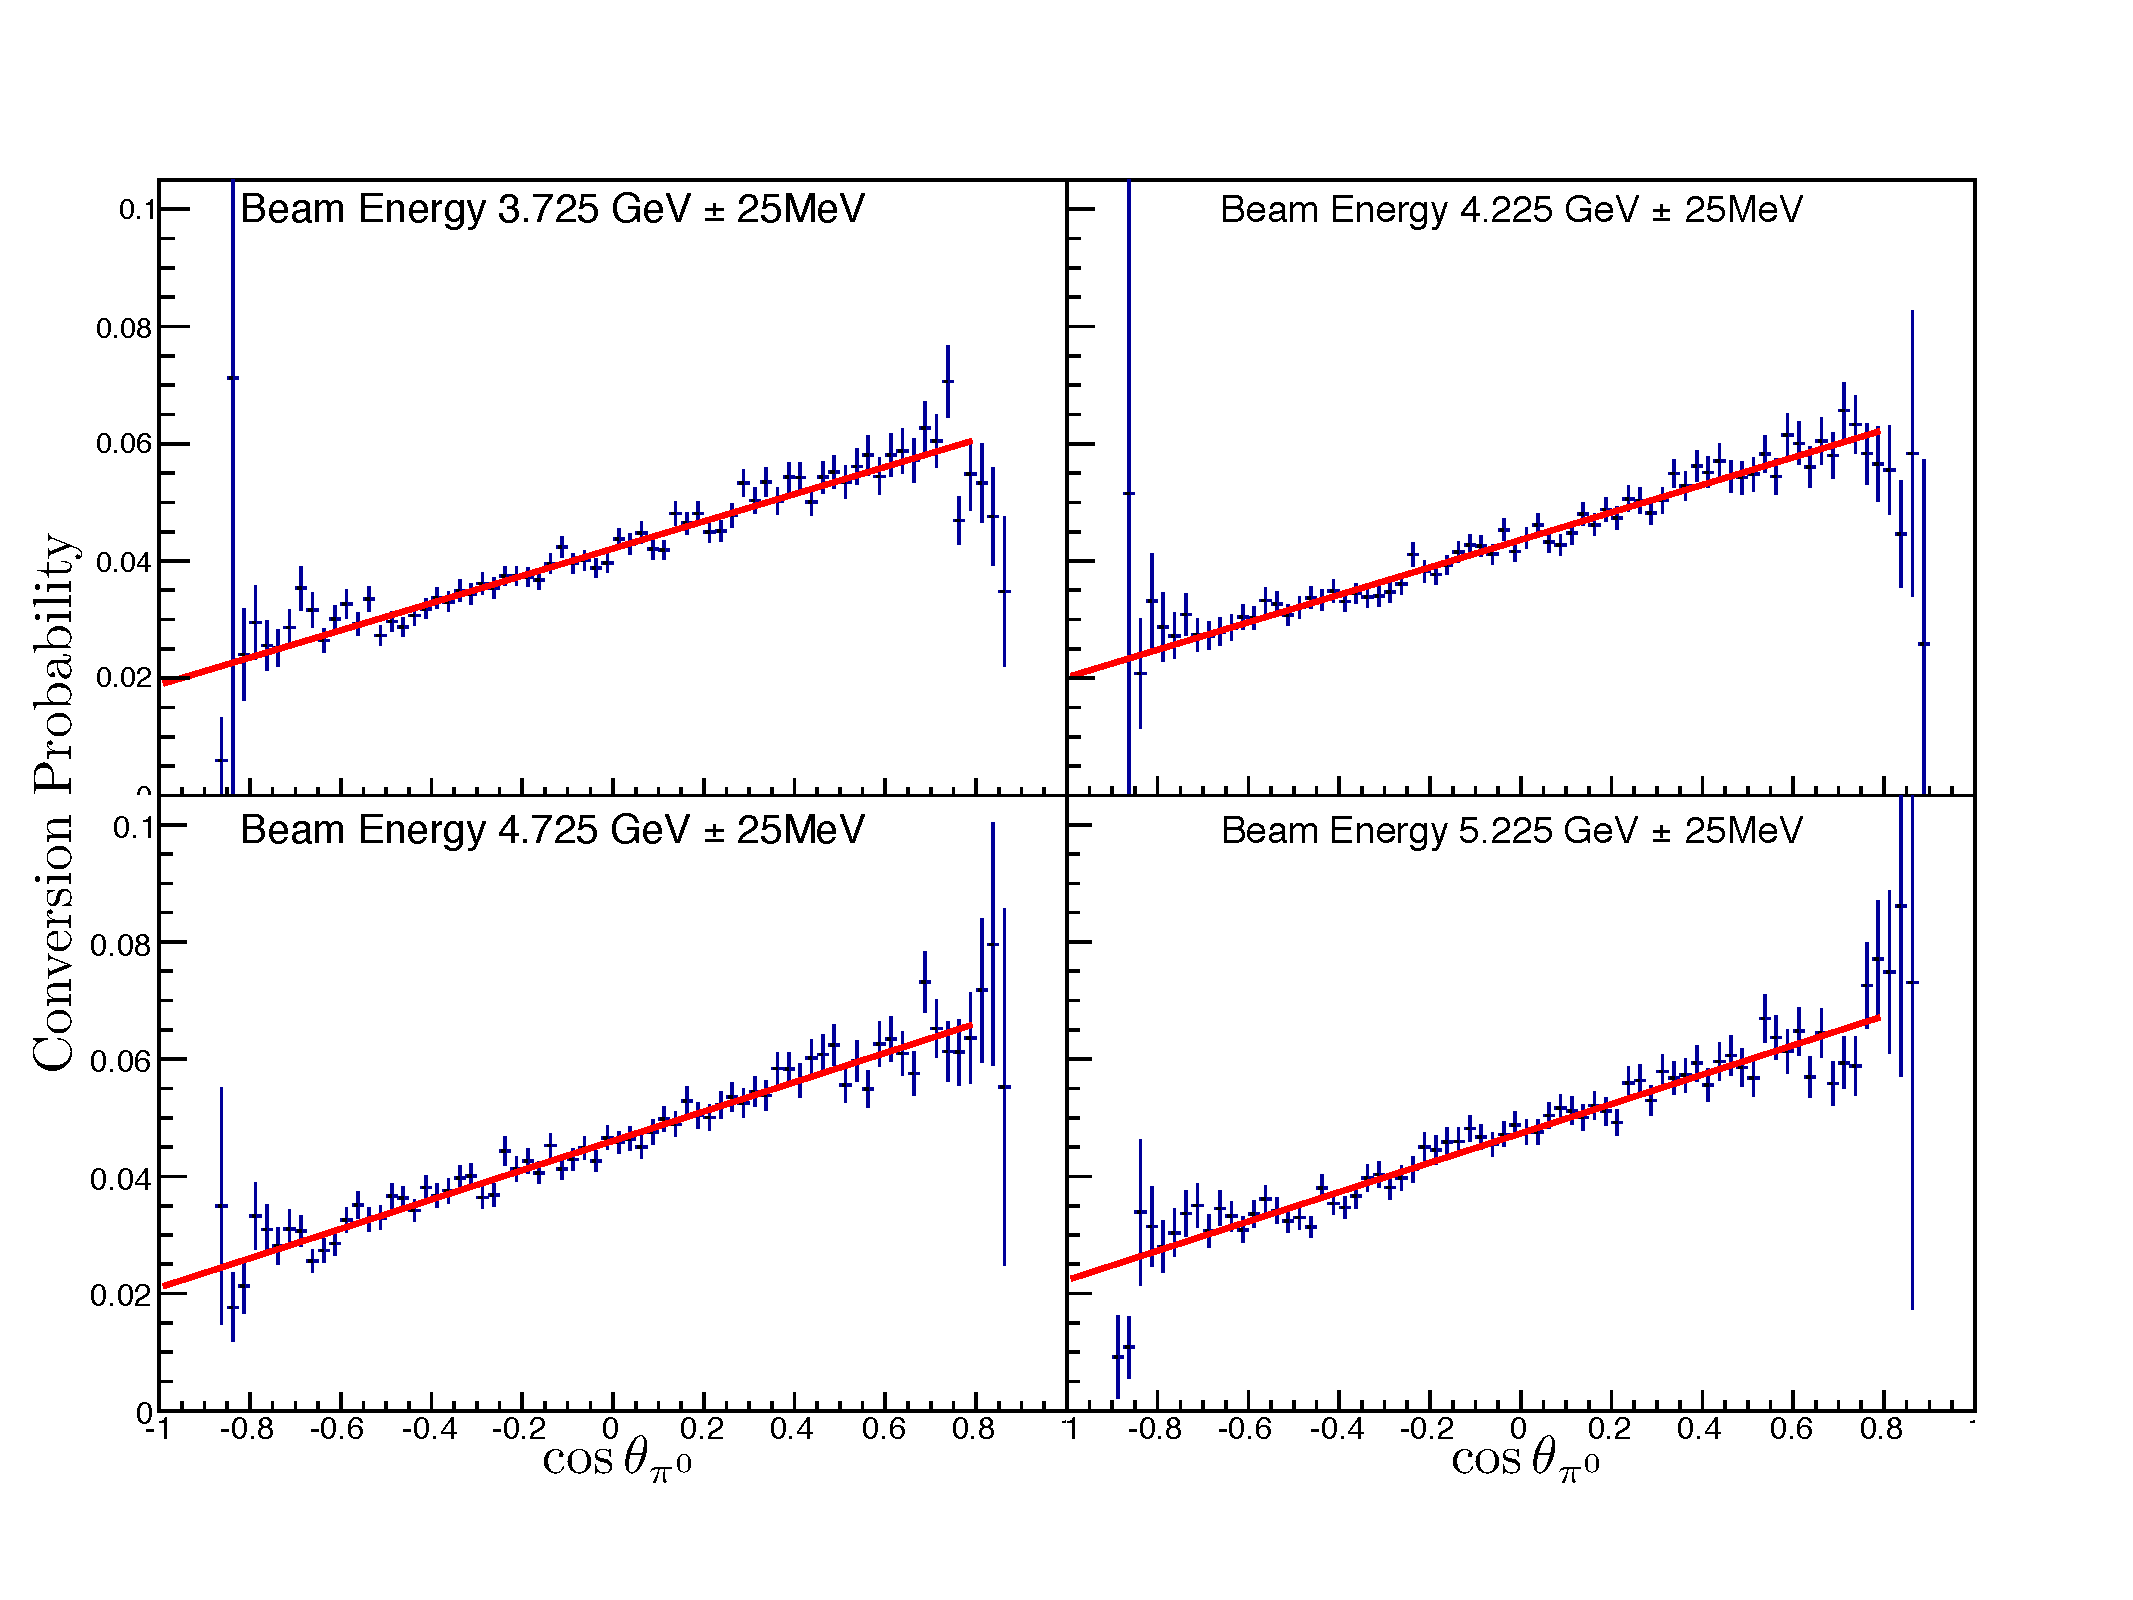
\includegraphics[width=\figwidth,height=\qfigheight]{\grpath/analysis/BRANCHING_RATIO/Converion_Probability_II_fix.pdf}\label{fig:convprob_II}
 		}
 		\caption[Probability of Photon Conversion vs. $\cos\theta$ for various values of $E_\gamma$]{\label{fig:convprob_all}Probability of Photon Conversion vs. $\cos\theta$ for various values of $E_\gamma$. The maximum probability for this analysis was measured in the top left plot of b.}
 	\end{center}\end{figure}
 	Therefore
 	\begin{align}
 		\frac{\Gamma}{\Gamma_{tot}} = \frac{\Gamma_{\pi^{0}\rightarrow e^{+}e^{-}\gamma}}{\Gamma_{tot}} + \frac{\Gamma_{\pi^{0}\rightarrow \gamma \gamma}P(\gamma \to  e^{+}e^{-})}{\Gamma_{tot}} = 0.09 \ ,
 	\end{align}
 	and has error
 	\begin{align}
 		\sigma_f = \sqrt{\left(\frac{1}{\Gamma_{tot}}\right)^2(\sigma^2_{\pi^{0}\rightarrow e^{+}e^{-}\gamma} + \sigma^2_{\pi^{0}\rightarrow \gamma \gamma})  } = 0.0037.  
 	\end{align}
 	The energy and $\cos \theta$ dependence of the conversion is accounted for in the acceptance, which is $E_\gamma$ and $\cos \theta$ bin-dependent. 
 	\begin{table}[h!]
\begin{minipage}{\textwidth}
\begin{center}


\caption[Branching Ratios of \piz]{\label{tab:brspecs}Branching ratio and errors used in $\frac{d\sigma}{d\cos\theta^{\pi^0}_{C.M.} d\phi}$ measurements \vspace{0.75mm}}

\begin{tabular}{c|c|c}

\hline
Quantity & Value & Error \\
\hline
$\Gamma_{\pi^{0}\rightarrow \gamma \gamma }$& 0.98823 & 0.00034 \\
$\Gamma_{\pi^{0}\rightarrow e^{+}e^{-}\gamma}$ & 0.01174 & 0.00035 \\
$\frac{\Gamma}{\Gamma_{tot}}$ & 0.13 & 0.0037 \\
\hline \hline
\end{tabular}


\end{center}
\end{minipage}
\end{table}
\vspace{20pt}
 	
 	
 	\subsection{Cut Based Systematic Uncertainty}
 	The procedure to determine the systematic uncertainty of the cuts placed on the various kinematic fits was first to calculate an acceptance with a different cut, then to calculate a new total cross-section measurement applying the different cut to the data. The total cross-section was computed at various photon beam energies. Lets denote the original measured total cross-section as $\Xi_1$ and the new total cross-section determined by the new cut as $\Xi_n$, then the systematic error was calculated as.
 	
 	\begin{align}
 		\sigma_{cut} = \frac{\left| \Xi_1 - \Xi_n \right|}{\Xi_1}
 	\end{align}
 	
 	Some systematic uncertainty depended on the photon energy. All cut based systematics were performed individually, meaning when a cut was changed, the remaining cuts retained their original value, see Table~\ref{tab:cutsystematics} for the values of the cuts that were changed to calculate the systematic error.
 	%This new cross-section was then compared to the cross-section using the base cuts to determine if a dependence on $\cos\theta^{\pi^0}_{C.M.})$ was present. All systematics of the cut based did not show a $\cos\theta^{\pi^0}_{C.M.})$ dependency for specific beam energies.
 	\begin{table}[h!]
\begin{minipage}{\textwidth}
\begin{center}


\caption[Variance of Data Cut Systematics]{\label{tab:cutsystematics}Different Cuts to analyze systematics \vspace{0.75mm}}

\begin{tabular}{c|c|c|c}

\hline
Cut & Original & Adjusted & Uncertainty \\
\hline
2-C Fit Pull Probability  & 1\% & 10\% & $0.0219$\\
1-C Fit Pull Probability & 1\% & 10\% & $ 0.00216 + 0.01083E_{\gamma}$ \\
4-C Fit Pull Probability  & 1\% & 10\% & $0.00031$\\
Missing Energy Cut  & 75~MeV & 100~MeV & $0.02781$\\
\hline \hline
\end{tabular}


\end{center}
\end{minipage}
\end{table}
\vspace{20pt}
 	
% 	\begin{figure}[h!]\begin{center}
% 			\includegraphics[width=1.2 \figwidth,height=\hfigheight]{\figures/analysis/All_Cut_Systematic.pdf}
% 			\caption[Plot showing the contribution of the data cut systematic error and the incoming beam dependence of the error]{\label{fig:sys_cut_error} Plot showing the contribution of the data cut systematic error and the incoming beam dependence of the error.}
% 		\end{center}\end{figure}

 		\subsection{Photon Flux Systematic Uncertainty}
 		The photon flux calculation should be consistent throughout the experiment. If the flux measurement is not consistent due to corrections made with the live-time, beam corrections or fractional difference in the reported current to the actual current during the photon flux normalization run then a systematic uncertainty would be produced. To study this effect we divided the g12 run period into four groups. Table~\ref{tab:flux_sys} lists the run groups used for this study.
 		\begin{table}[h!]
\begin{minipage}{\textwidth}
\begin{center}


\caption[Run Groups Used to Determine Photon Flux Systematic Error ]{\label{tab:flux_sys}List of run groups used to determine photon flux systematic error. \vspace{0.75mm}}

\begin{tabular}{c|c|c}

\hline
Run Group & Range & Total Runs \\
\hline
1 & 56605-56798 & 116 \\
2 & 56799-56980 & 116 \\
3 & 56992-57173 & 116 \\
4 & 57174-57317 & 115 \\
\hline \hline
\end{tabular}


\end{center}
\end{minipage}
\end{table}
\vspace{20pt}
 		
 		The procedure to determine the systematic error, $\sigma$, of the flux is to calculate the accepted and flux corrected yield, $\Upsilon^c$, for each run group and compare $\Upsilon^c$ to the average accepted and flux corrected yield of all 4 run groups, $\mu^c$. After $\sigma$ is calculated, it was normalized to $N \mu^c$ as to represent the error as a percentage, which later is added in quadrature and  multiplied by the measured cross section to determine the appropriate error. 
 		\begin{align}
 			\sigma_{group} = \sqrt{\sum_{i=1}^{N = 4}\left(\Upsilon_i^c - \mu^c\right)},
 		\end{align}
 		where
 		\begin{align}
 			\mu^c = \frac{1}{N}\sum_{i=1}^{N=4}\Upsilon_i^c
 		\end{align}
 		\begin{align}
 			\sigma_{group}^{normalized} = \frac{\sigma_{group}}{N\mu^c}
 		\end{align}
 		
% 		\begin{figure}[h!]\begin{center}
% 				\includegraphics[width=1.2 \figwidth,height=\hfigheight]{\figures/analysis/Beam_Fluxsystematic_Error.pdf}
% 				\caption[Plot showing the contribution of the flux systematic error and the incoming beam dependence of the error]{\label{fig:sys_flux_error} Plot showing the contribution of the flux systematic error and the incoming beam dependence of the error.}
% 			\end{center}\end{figure}

 			
 			
 			
 			\subsection{Detector Efficiency Systematic Uncertainty}
 			Each sector in \abbr{CLAS} can be treated as an individual detector, with its own efficiency and resolution. A systematic uncertainty could arise if one or more of the sectors is not simulated properly. The procedure to determine the systematic error, $\sigma$, of the sector is to calculate the accepted corrected yield, $\Upsilon^c$, for each sector and compare $\Upsilon^c$ to the average accepted corrected yield of all 6 sectors, $\mu^c$. After $\sigma$ is calculated, it was normalized to $N \mu^c$ as to represent the error as a percentage, which later is multiplied by the measured cross section to determine the appropriate error. 
 			\begin{align}
 				\sigma_{sector} = \sqrt{\sum_{i=1}^{N = 6}\left(\Upsilon_i^c - \mu^c\right)},
 			\end{align}
 			where
 			\begin{align}
 				\mu^c = \frac{1}{N}\sum_{i=1}^{N=6}\Upsilon_i^c
 			\end{align}
 			\begin{align}
 				\sigma_{sector}^{normalized} = \frac{\sigma_{sector}}{N\mu^c}
 			\end{align}
 			This calculation was performed for various bins of incoming beam energy to determine the beam energy dependence.% (see Fig.~\ref{fig:sys_sec_error}).
 			
% 			\begin{figure}[h!]\begin{center}
% 					\includegraphics[width= \figwidth,height=0.75\hfigheight]{\figures/analysis/Beam_systematic_Error.pdf}
% 					\caption[The sector systematic uncertainty as a function of the incoming photon energy]{\label{fig:sys_sec_error}The sector systematic uncertainty as a function of the incoming photon energy.}
% 				\end{center}\end{figure}
 				%The sector systematic uncertainty is consistent with the extracted sector systematic uncertainty from the g11 data set~\cite{williams}(seeFig.~\ref{fig:sys_sec_error.compare}).
% 				\begin{figure}[h!]\begin{center}
% 						\includegraphics[width= \figwidth,height=0.75\hfigheight]{\figures/analysis/S_systematic_Error.pdf}
% 						\caption[Comparison of sector systematic uncertainty to g11 measurement]{\label{fig:sys_sec_error.compare}Comparison of sector systematic uncertainty to g11 measurement.}
% 					\end{center}\end{figure}

 					
 					\subsection{$z$-vertex Cut Systematic Uncertainty}
 					The systematic uncertainty of the $z$-vertex cut was analyzed by varying the initial vertex cut from $-110 \le z \le -70$ to $-109 \le z \le -71$ for both data and \abbr{MC}. Afterward the procedure for determining the systematic was identical to the method used to determine the ``Cut Based Systematic Uncertainty". The systematic uncertainty from varying the $z$ was 0.0041, shown in Fig.~\ref{fig:results.syserr}
 					
 					\subsection{Target Systematic Uncertainty}
 					Since the systematic on the density is 0.02\%,see Sec~\ref{sec:analysis.target_density}, the maximum systematic on the target is due to uncertainty in the length on the target which is 40~cm $\pm$ 0.2~cm. A total systematic on the target was assign to be 0.5\%. 
 					
 					\subsection{Total Systematic Uncertainty}
 					The total systematic uncertainty along with a list of the individual systematics is presented in this subsection. The calculation of the total systematic error is 
 					\begin{align}
 						\sigma^{sys}_{tot} = \sqrt{\sum_{i=1}^{M}\sigma_i^2}
 					\end{align}
 					\begin{table}[h!]
\begin{minipage}{\textwidth}
\begin{center}


\caption[Systematics]{\label{tab:systematics}Systematic errors used in $\frac{d\sigma}{d\cos\theta^{\pi^0}_{C.M.} d\phi}$ measurements \vspace{0.75mm}}

%\begin{tabular}{c|c}
\begin{tabular}{p{5cm} | p{7cm}}
\hline
Systematic & Error \\
\hline
Sector  & $ 0.0361 + 0.0065E_{\gamma}$ \\
Flux  & $ -0.00051 + 0.00491E_{\gamma}$ \\
Missing Energy Cut  & $0.02781$ \\
2-C Fit Pull Probability & $0.0219$ \\
1-C Fit Pull Probability  & $ 0.00216 + 0.01083E_{\gamma}$ \\
4-C Fit Pull Probability  & $0.00031$ \\ 
Target  & $0.005$ \\
Branching Ratio  & $0.0037$ \\
Fiducial Cut & $0.024$ \\
$z$-vertex Cut & $0.0041$ \\
Total & $\sqrt{0.0032 +0.00051E_{\gamma} +0.000184E_{\gamma}^2}$ \\
\hline \hline
\end{tabular}


\end{center}
\end{minipage}
\end{table}
\vspace{20pt}
% 					Figure~\ref{fig:results.syserr} is a pictorial version of Table~\ref{tab:systematics}.
% 					\begin{figure}[h!]\begin{center}
% 							\includegraphics[width=1.1 \figwidth,height=\hfigheight]{\figures/analysis/All_Systematics_new.pdf}
% 							\caption[The contribution of all systematic uncertainties]{\label{fig:results.syserr}The contribution of all systematic uncertainties.}
% 						\end{center}\end{figure} 
%\section{\label{sec:level1}Normalization}
Write 
%\section{\label{sec:level1}Cross-Sections}
Write 
\section{\label{sec:level1}Comparison with Theoretical Models}
There are several models that attempt to describe  $\pi^0$ photoproduction in the low beam energy resonance region, while in the high beam energy regime there exists limited amount of theory. Described below are two theories. 
\subsubsection{Regge Theory}
Another approach to describe the production of the \piz meson in photoproduction is to use Regge theory. According to Regge theory the reaction amplitudes can be described by Regge poles in which the dominant Regge poles originate from t-channel exchange. This model has been developed over the years and is greatly described in~\cite{JPAC}. Using this model along with the \g12 measurements, seen in figure~\ref{fig:pi0_regge}, it is shown that this theory provides a good description of the data obtained by \g12 and a previous measurement~\cite{brem}.
\begin{figure}[h]
	\centerline{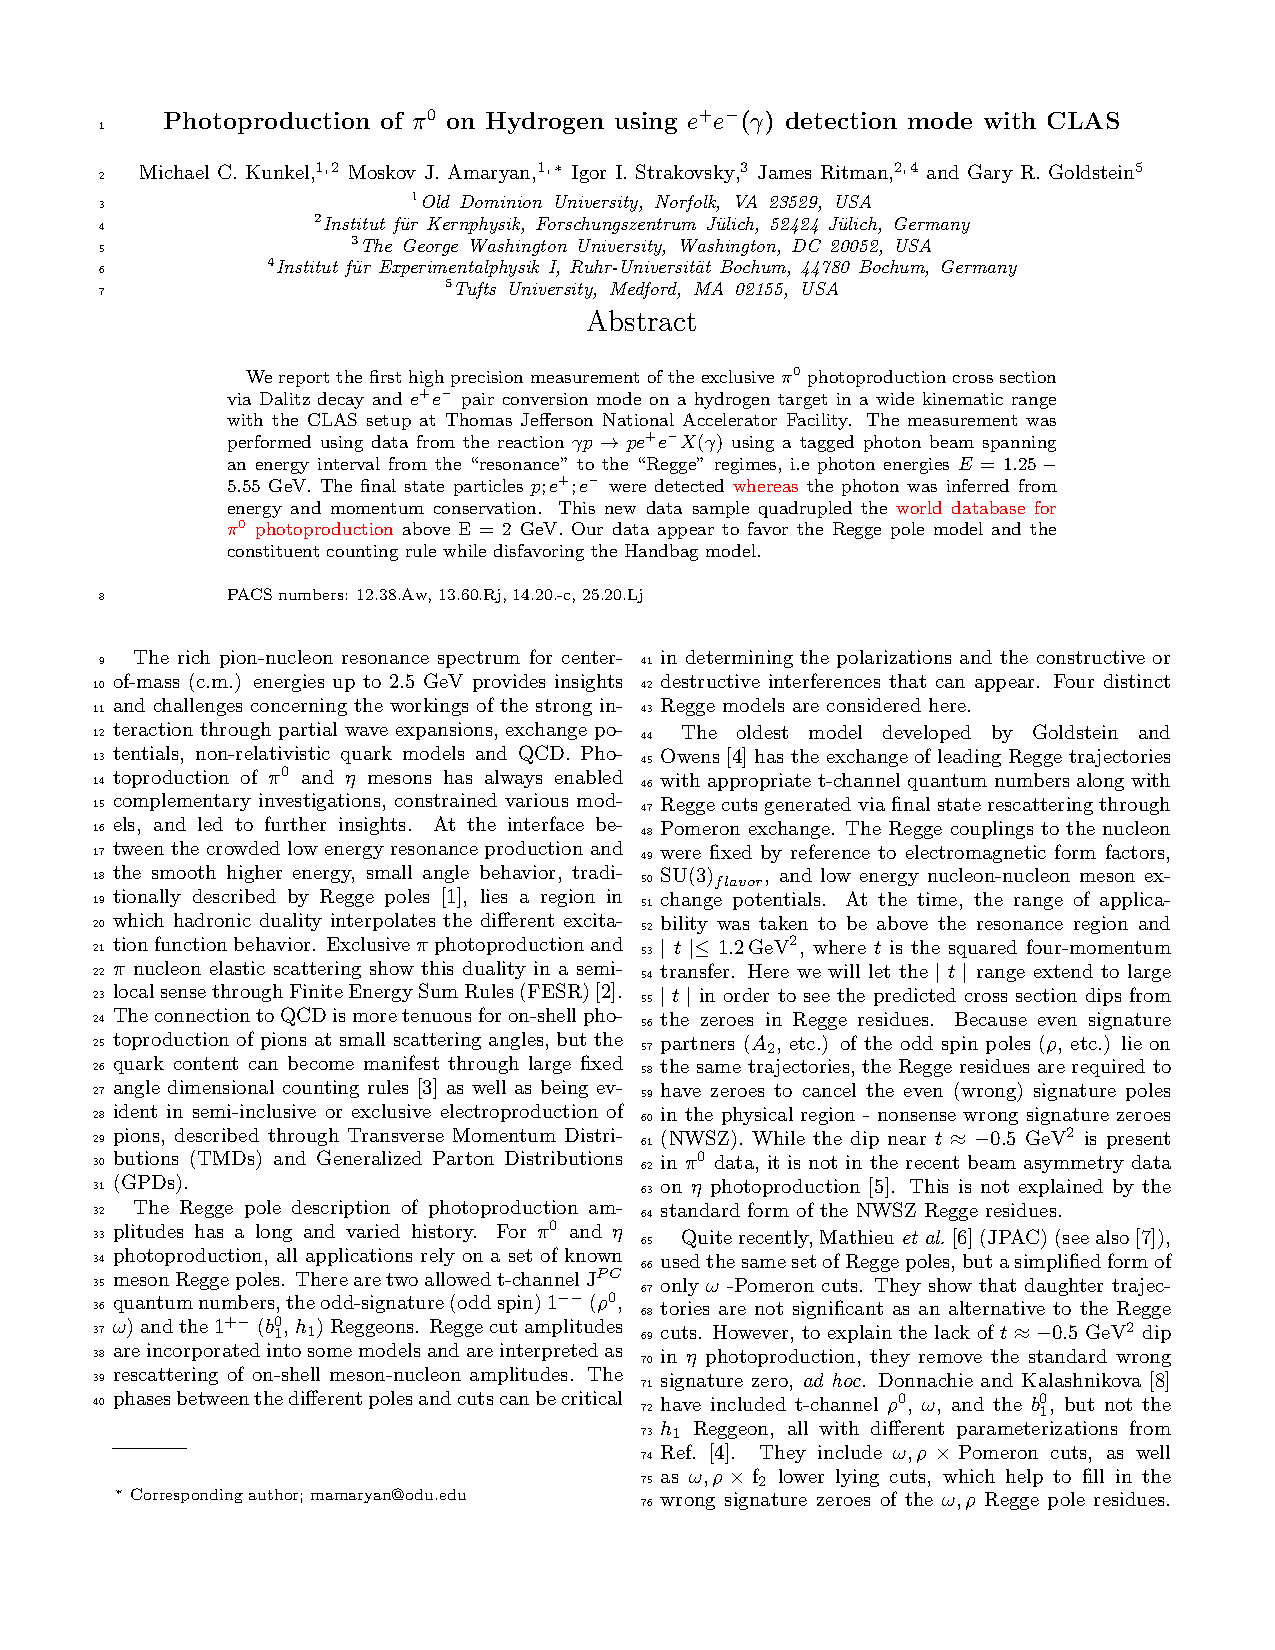
\includegraphics[width=275 pt, height = 160 pt]{\figures/analysis/DSG/pi0_regge.pdf}}
	\caption{Comparison with Regge model. Experimental data are from the current measurement (red filled circles) and previous bremsstrahlung measurements~\protect\cite{brem} (black open circles). }
	\label{fig:pi0_regge}
\end{figure}
\section{\label{sec:summary}Summary}

\nocite{*}
\bibliographystyle{aipnum-cp}%
\bibliography{PI0}%
%
% ****** End of file apssamp.tex ******
\end{document}